\documentclass[10pt,a4paper]{article}
\usepackage[english]{babel}
\usepackage[utf8]{inputenc}
\usepackage{amsmath}
\usepackage{amsfonts}
\usepackage{amssymb}
\usepackage{graphicx}
\usepackage{caption}
\usepackage{subcaption}
\usepackage{url}
\usepackage{fullpage}
\author{Joan Puigcerver i Pérez\\
\begin{footnotesize}
\emph{joapuipe@upv.es}
\end{footnotesize}}
\title{Handwritten Text Recognition Using Conditional Random Fields}
\begin{document}
\maketitle

\section{Introduction}
Handwritten text recognition (HTR) has been broadly studied in the literature by pattern recognition and computer vision researchers. However it is still far from being solved, mainly due to the high variability that involves the handwritten text in comparison to other forms of text (printed text, for instance) or other signals. In some domains, good results have been achieved for both online and offline text recognition using Hidden Markov Models (HMMs) and $n$-grams Language Models (LM). HMMs are typically used to model the morphology of the characters and LMs are used to combine different HMMs of characters to build complete words and sentences. Despite the latest success of HMMs in HTR, Conditional Random Fields (CRFs)\cite{lafferty2001conditional} have been shown better to label sequential data over HMMs in many other areas like part-of-speech tagging, name entity recognition, parsing, gene finding, etc.\\

Here we present an alternative to HMMs for offline sentence-level handwritten text recognition using CRFs. This work is inspired by previous work present in the literature\cite{feng2006exploring} and aims to be an initial work to explore the use of CRFs for HTR.

\section{Conditional Random Fields}
CRFs are undirected graphical models that allow to compute the probability of label sequences given (conditioned to) a sequence observation. $O = \vec{o}_1, \vec{o}_2, \ldots, \vec{o}_T$ denotes the sequence of vector observations and $S = s_1, s_2, \ldots, s_T$ denotes the sequence of labels or states. Here we assume that the length of the observed sequence is equal to the length of the label sequence. According to CRF formulation, the conditional probability $P(S|O)$ is modelled by:\\

\begin{equation}\label{eq:general_crf}
P(S|O) \approx P_\theta(S|O) = \frac{1}{Z_\theta(O)} \exp \left( \sum_{k=1}^K \lambda_k f_k(S,O) \right)
\end{equation}

Equation \ref{eq:general_crf} shows the general equation for CRFs, where $\{f_k\}_{k=1}^K$ is a set of boolean feature functions defined on $f_k : \mathbb{S}^T \times \mathbb{O}^T \rightarrow \{0,1\}$ with its associated set of weights $\{\lambda_k\}_{k=1}^K$. $Z_\theta(O)$ is a normalization factor over all possible labelling for the given observation sequence:\\

\begin{equation}
Z_\theta(O) = \sum_{S' \in \mathbb{S}^T} \exp \left( \sum_{k=1}^K \lambda_k f_k(S',O) \right)
\end{equation}

To reduce the complexity of the model the first-order Markov assumption is usually taken, resulting in a linear-chain CRF with the following equation to model $P(S|O)$.\\

\begin{equation}
P_\theta(S|O) = \frac{1}{Z_\theta(O)} \exp \left( \sum_{t=1}^T \sum_{k=1}^K \lambda_k f_k(s_{t-1},s_t,O,t) \right)
\end{equation}

Finally, it is also assumed that the probability of a given observed vector at time $t$ only depends on state $s_t$ and the transition probability from $s_{t-1}$ to $s_t$ does not depend on $O$, which results in the final formula that we used to model $P(S|O)$, showed in equation \ref{eq:linear_crf}.\\

\begin{equation}\label{eq:linear_crf}
P_\theta(S|O) = \frac{1}{Z_\theta(O)} \exp \left( \sum_{t=1}^T \left( \sum_{k=1}^K \lambda_k f_k(s_t, \vec{o}_t) + \sum_{l=1}^L \mu_l g_l(s_{t-1}, s_t)\right) \right)
\end{equation}

The normalization term $Z_\theta(O)$ can be then rewritten as:\\
\begin{equation}\label{eq:Z_linear_crf}
Z_\theta(O) = \sum_{S' \in \mathbb{S}^T} \exp \left( \sum_{t=1}^T \left( \sum_{k=1}^K \lambda_k f_k(s'_t, \vec{o}_t) + \sum_{l=1}^L \mu_l g_l(s'_{t-1}, s'_t)\right) \right)
\end{equation}

This simplification reduces the number of parameters from $O(2^{|\mathbb{S}| |\mathbb{O}|})$. present in equation \ref{eq:general_crf}, to $O(|\mathbb{S}|^2 + |\mathbb{S}||\mathbb{O}|)$, in equation equation \ref{eq:linear_crf}. This simplification reduces not only the amount of data needed to train the CRFs but also the computational complexity of the decoding and training process.\\

Viterbi algorithm is used to find the labels sequence $\hat{S}$ which gives the highest probability $P_\theta(\hat{S}|O)$, given the observed sequence of vectors. The CRF parameters ($\theta = \{\lambda_k \}_{k=1}^K \cup \{\mu_l\}_{l=1}^L$) are trained by minimizing the following loss function $\mathcal{L}$. This is typically done using L-BFGS method. Any optimization method can be used such as gradient descent or other quasi-Newton methods like L-BFGS, but the later is usually preferred since it provides a faster convergence.\\

\begin{equation}\label{eq:crf_loss}
\mathcal{L} = \sum_{n=1}^N\log(P_\theta(S^{(n)} | O^{(n)})) - \frac{1}{2C} \left( \sum_{k=1}^K \lambda_k^2 + \sum_{l=1}^L \mu_l^2 \right)
\end{equation}

Hyperparameter $C$ is a cost term added to control the regularization of the model. With high values for $C$, the model tends to overfit the training data. 


\section{CRF feature functions}\label{sec:feature_funcs}
The definition of the feature functions $g_l$ in our scenario is straight, given a label sequence S.\\

\begin{equation}
g_l(s_{t-1}, s_{t}) = \begin{cases}
1 & \text{if } s_{t-1} = w_{l} \wedge s_{t} = w'_{l}\\
0 & \text{otherwise}
\end{cases}
\end{equation}

The variables $w_{l}$ and $w'_{l}$ represent two words in the training vocabulary. Note that there are $O(V^2)$ feature functions $g_l$ (one for each pair of words in the training vocabulary). Note also that $V = \mathbb{S}$.\\

The feature functions $f_k$ are defined using the state $s_t$ and the observation vector $\vec{o}_t$. If no independence is assumed among the dimensions of the observation vector, this would lead to $O(|\mathbb{B}|^D |\mathbb{S}|)$ feature functions $f_k$, where $D$ is the dimensionality of the observation vector and $\mathbb{B}$ is the set of values that each dimension of the observation vector can take. In order to simplify the model, we will define $\{f_{k,d}\}_{d=1}^D$ a set of feature function, where each function $f_{k,d}$ has the following form.\\

\begin{equation}
f_{k,d}(s_t, o_{t,d}) = \begin{cases}
1 & \text{if } s_{t-1} = w_k \wedge o_{t,d} = v_{k,d} \\
0 & \text{otherwise}
\end{cases}
\end{equation}

The variable $w_k$ represents a word in the training vocabulary $V$ and $v_{k,d}$ represents a discrete value in $\mathbb{B}$. So, the number of features is reduced to $O(D |\mathbb{B}| |\mathbb{S}|)$. The resulting number of parameters of the CRF model to be estimated is $O(D |\mathbb{B}| |\mathbb{S}| + |\mathbb{S}|^2)$.

\section{Observation features}
As we explained before, each observation will be a sequence of vectors $\vec{o}_t$. Each of these vectors is a set of features extracted from a segmented word image from a text line to be recognized. In the state-of-the-art systems, the number of feature vectors depends usually on the length of the image, but here we are using just one vector to represent the whole word image. All the feature extraction process have been done to mimic the previous work published by other authors in the field\cite{feng2006exploring,lavrenko2004holistic}, except the estimation of the number of ascenders and descenders, which was not explained in the referred papers.\\

From each word image, the following six scalar features are extracted:\\
\begin{itemize}
\item Height of the image ($h$)
\item Width of the image ($w$)
\item Aspect ratio ($\frac{w}{h}$)
\item Image area ($w \cdot h$)
\item Estimated number of descenders in the word (``\emph{field}'' would have one descendent, corresponding to the lower part of the character \emph{f})
\item Estimated number of ascenders in the word (``\emph{field}'' would have three ascenders: the upper part of the \emph{f}, \emph{l} and \emph{d})
\end{itemize}

To compute an approximation of the number of ascenders and descenders, first the ascenders and descender lines are approximated using the method described in \cite{gadea2007aportaciones}. Then, the ``skeleton'' of the text image is computed and the number of ascenders and descenders is estimated as the number of intersections through the ascender and descender lines. An example of this procedure can be shown in figure \ref{fig:img_features_ascdes}.\\

Additional features based on the shape of the actual handwritten text are also used. We compute the upper word profile (maximum y-coordinate of the foreground pixels in each column, see figure \ref{fig:img_features_upper}), the lower word profile (minimum y-coordinate of the foreground pixels in each column, see figure \ref{fig:img_features_lower}) and the projection profile (percentage of foreground pixels in each column, see figure \ref{fig:img_features_project}) of each word image and then we extract the first 4 real components and the first 3 imaginary components from the Discrete Fourier Transform of each of this profiles. This gives us $7 \times 3 = 21$ scalar features extracted from the profiles.\\

All the previous 27 scalar features are real numbers that cannot be handled easily by CRFs. In order to discretize these continuous features, two binning schemes are used. The first discretizes each dimensions of the 27-continuous vector into 10 bins, while the second discretizes each dimension into 9 bins. Thus, a final discrete 54-dimensional feature vector is extracted from each word image.\\

\begin{figure}[h]
\centering
\begin{subfigure}[b]{0.45\textwidth}
\centering
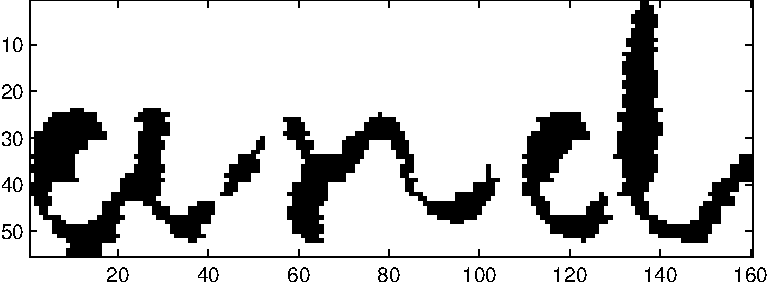
\includegraphics[width=\textwidth]{imgs/and_orig-crop.pdf}
\caption{Original image from the Washington corpus.}
\label{fig:img_original}
\end{subfigure}
~
\begin{subfigure}[b]{0.45\textwidth}
\centering
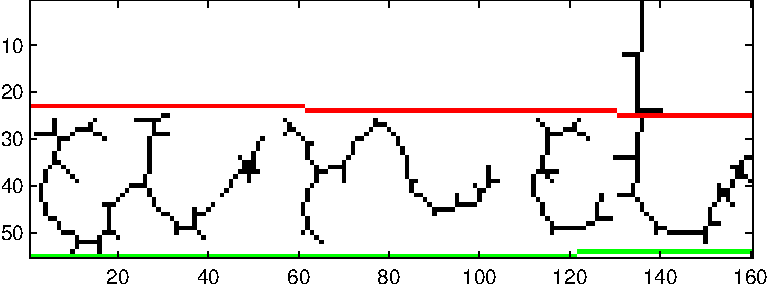
\includegraphics[width=\textwidth]{imgs/and_asc_des-crop.pdf}
\caption{Detected ascenders (red) and descenders lines (green).}
\label{fig:img_features_ascdes}
\end{subfigure}
\\
\begin{subfigure}[b]{0.45\textwidth}
\centering
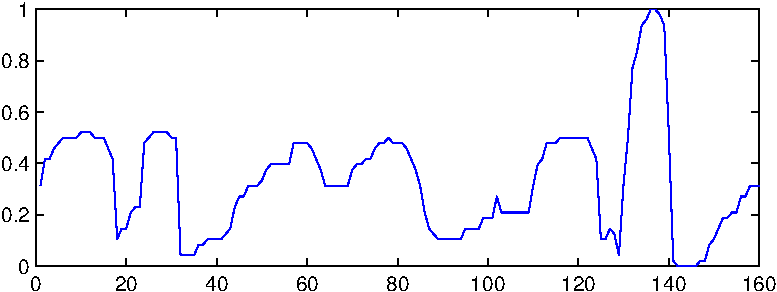
\includegraphics[width=\textwidth]{imgs/and_upper-crop.pdf}
\caption{Upper-word profile from the original image.}
\label{fig:img_features_upper}
\end{subfigure}
~
\begin{subfigure}[b]{0.45\textwidth}
\centering
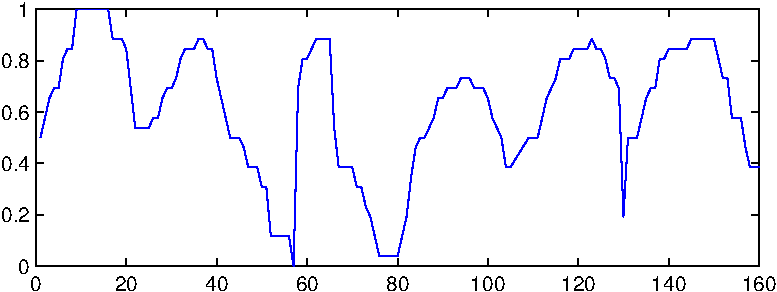
\includegraphics[width=\textwidth]{imgs/and_lower-crop.pdf}
\caption{Lower-word profile from the original image.}
\label{fig:img_features_lower}
\end{subfigure}\\
\begin{subfigure}[b]{0.45\textwidth}
\centering
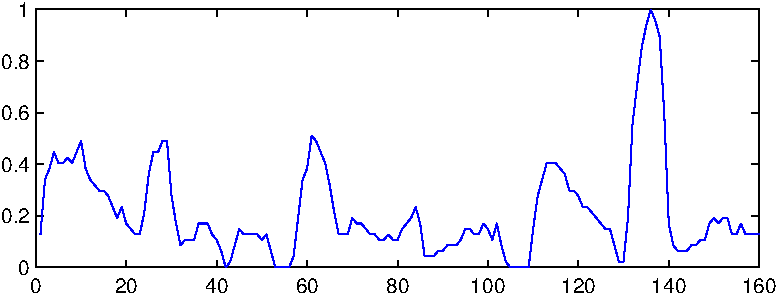
\includegraphics[width=\textwidth]{imgs/and_projection-crop.pdf}
\caption{Projection profile from the original image.}
\label{fig:img_features_project}
\end{subfigure}
\caption{Different processing steps over an example image from the Washington corpus\cite{fischer2012lexicon}.}
\label{fig:img_features}
\end{figure}

\section{Experiments}
The experiments described in this section were done using the Washington Database collected by the Research Group on Computer Vision and Artificial Intelligence (FKI) from the University of Bern\cite{fischer2012lexicon}. The database contains 20 pages from the original Washington Letters corpus released by the Library of Congress of the United States which were cleaned, normalized, binarized and word-segmented by the FKI group. The statistics of each partition is described in table \ref{tab:data}. The validation set from the first partition (CV1) was used to tune the hyperparameters of the CRF models (the regularization term $C$, introduced in equation \ref{eq:crf_loss}). Each partition includes its own test set, so the final system was trained using the train and validation sets (Tr+Va column) from each partition and the errors reported on the test set for each partition were averaged.\\

\begin{table}[h]
\centering
\begin{tabular}{|c|c|c|c|c|c|c|c|c|}
\hline
 & \multicolumn{4}{|c|}{Sentences} & \multicolumn{4}{|c|}{Vocabulary} \\
\hline
Partition & Train & Valid & Tr+Va & Test & Train & Valid & Tr+Va & Test \\
\hline
CV1 & 325 & 168 & 493 & 163 & 835 & 606 & 1238 & 525 \\
CV2 & 329 & 163 & 492 & 164 & 950 & 525 & 1224 & 529 \\
CV3 & 331 & 164 & 495 & 161 & 946 & 529 & 1232 & 495 \\
CV4 & 327 & 161 & 488 & 168 & 865 & 495 & 1122 & 606 \\
\hline
\end{tabular}
\caption{Summary of the four partitions from the Washington Database used to perform the described experiments. Vocabulary is the number of different words in each set.}
\label{tab:data}
\end{table}

The performance of the system is given using the word accuracy ($\frac{C}{N}$, where $C$ is the number of correctly labeled word images and $N$ is the total number of images). Since the word-segmentation of each line is given, no insertions or deletions can happen, so the popular WER measure is not needed in this scenario.\\

In order to build the CRFs models, CRF++ toolkit\footnote{\url{https://code.google.com/p/crfpp/}} was used. The optimization of the loss function described in equation \ref{eq:crf_loss} was stopped when the relative improvement of the loss function was under 0.001 points. Table \ref{tab:results_valid} shows the results of different CRFs models trained with different regularization constants $C$ on the validation set from CV1. The number of effective feature functions used was 1082995 (feature functions evaluated to 1 by some training sentence), which represents about 96.2\% of all possible feature functions (1125580) that can be defined as described in section \ref{sec:feature_funcs}. If this percentage were much lower, the model would have a high risk of over-fitting. Table \ref{tab:results_valid} also shows that no over-fitting is observed for the explored $C$ values (the higher $C$, the higher risk of over-fitting).\\

\begin{table}[h]
\centering
\begin{subfigure}[b]{0.45\textwidth}
\centering
\begin{tabular}{|c|c|}
\hline
$C$ & Accuracy\\
\hline
$10^{-2}$ & 0.221964 \\
$10^{-1}$ & 0.361176 \\
$10^0$ & 0.401392 \\
$10^1$ & 0.408353\\
$10^2$ & 0.410673\\
$10^3$ & 0.411446\\
$10^4$ & 0.415313\\
\hline
\end{tabular}
\caption{Accuracy on the validation set of the CV1 partition.}
\label{tab:results_valid}
\end{subfigure}
~
\begin{subfigure}[b]{0.45\textwidth}
\centering
\begin{tabular}{|c|c|}
\hline
Partition & Accuracy\\
\hline
CV1 & $0.520548$\\
CV2 & $0.531605$\\
CV3 & $0.526272$\\
CV4 & $0.449343$\\
\hline
Average & $0.506942 \pm 0.037891$\\
\hline
\end{tabular}
\caption{Accuracy on the test set of each partition and the averaged accuracy with 95\% confidence interval.}
\label{tab:results_test}
\end{subfigure}
\caption{}
\end{table}

The final model was trained as explained before for each partition and the final results on the test set are shown in table \ref{tab:results_test}. Since training each CRF model is expensive in terms of computation time, the maximum number of optimization iterations was set to 50. Each model needed about 3 hours to train in a 3.2Ghz Intel Core i7, using 8 threads to train the model. The cost of training the same model in a single core would be around 24 hours. The averaged accuracy on the test sets is $\mathbf{0.506942 \pm 0.037891}$.

\section{Conclusions}
The use of CRFs for handwritten text recognition was explored using image features and CRF feature functions similar to the used in previous works\cite{feng2006exploring}. The results achieved in this work are much better than the previously reported (0.428), but there are some details in the referenced work that are not known and may explain the difference: we are not completely sure that the pages used from the Washington database are the same, we also do not know if the images have been preprocessed in the same way (in terms of noise reduction, normalization and binarization). We also detailed the procedure that we followed to estimate the number of ascenders and descenders, but the previous work does not explain or reference their procedure to estimate these image features.\\

The major problems of the current approach is that it requires explicit segmentation, while most of current HTR systems based on HMMs deal with the word segmentation implicitly with the decoding. This is a tremendous advantage since word segmentation is not always easy to do using automatic approaches for handwritten images, and the manual segmentation needs too much human resources for large projects.\\

It would be also interesting to reduce the number of states (and hence, parameters) of the CRFs by using character-based instead of word-base CRF. This would dramatically reduce the number of states to a few dozens, but probably would require a higher-order Markov assumption to achieve good results. Some attempts in this direction have already been done in the literature\cite{shetty2007handwritten}, but they rely on the explicit segmentation of characters, which is even more difficult and problematic for HTR than word segmentation.\\

\bibliographystyle{abbrv}
\bibliography{htrcrf}

\end{document}